\documentclass[10pt, letterpaper, twocolumn]{article}
\usepackage[margin=1in]{geometry}
% Use CC style guide fonts rather than default fonts
\usepackage{fontspec} 
\usepackage{graphicx}
\setmainfont[Ligatures=TeX]{Crimson}
\setsansfont[Ligatures=TeX]{Montserrat}
\begin{document}
\twocolumn[ \centerline{\Huge
%%%% Title
CP341: Reinventing the Internet
}
\vspace{1cm}
\centerline{
%%%% Team of 3 authors block
\begin{tabular}{ccc}
Evelyn Needham & Oliver Kendall \\
e\_needham2023@coloradocollege.edu & o\_kendall@coloradocollege.edu\\
\end{tabular}
%%%% Team of 4 authors block
%\begin{tabular}{cc}
%Alex the Bear & Laurie Sloth \\
%alex@dellswor.net & laurie@dellswor.net \\
%\\
%Danielle Ellsworth & Leapord \\
%dellsworth@coloradocollege.edu & \\
%\end{tabular}
\vspace{1cm}
} ]

\begin{abstract}
Today, the Internet and the varied components and layers that make it up are taken as a given. Everything is abstracted from the user, allowing them to never confront what it actually is that allows them to send cat videos halfway across the world. This abstraction makes the Internet accessible to anyone, requiring zero background or knowledge in computing. Yet, it also means that alternative approaches to the fundamental questions of network engineering are rarely considered. Prior to 3.5 weeks ago, neither of us had ever stopped and thought about these very questions. Quite frankly, neither of us had stepped out of a world of high-level, abstracted programming languages and picked up a piece of hardware. This paper will recount our process of building up a functioning network from basic hardware components and mini, inexpensive Raspberry Pi computers programmed in C. In its current configuration, it can support up to 5 NIC-pi pairs that one has access to, with all of them essentially running the same software. This limitation is a result of our chosen network topology and the number of ports (4) on each NIC (it can support n+1 machines where n is the number of ports on a network card). Its current form does require the user to manually input information about each computer necessary for the network layer as well as the destination for one’s input (message for chat feature or game move for battleship). This is hardcoded into the network layer. If we had more time, this would be the first upgrade we would make to our network, allowing it to be far more dynamic, extendable, and resistant to structural changes, such as destroyed connections. 
\end{abstract}

\section{Introduction}
This paper recounts and describes our attempts to reinvent the Internet in 3.5 weeks. The tools provided to us were Raspberry Pis, custom, hand-soldered network interface controllers (NICs), ribbon cables to connect the two, and optical cables to connect Raspberry Pi/NIC pairs. The general novelty of our setup allowed for infinite freedom as there were no existing strategies or conventions using these tools. However, this same novelty of solving an unsolved problem meant that there were few answers to our many questions. Luckily, there are a plethora of resources to answer the larger and more conceptual questions as the Internet has already been invented. These are questions like: how can one send any kind of information when their only capability is turning a switch on or off? Or: how does data know how to get to its final destination if not directly connected? The vast amounts of research we did could not build a network itself, but guided us through our creation. This paper walks through the basics of computer network engineering, our design choices and implementation, how we arrived at these, the challenges we faced, and what we build off of and improve if given more time. 

\section{Approach}
\begin{figure}[ht]
\centering
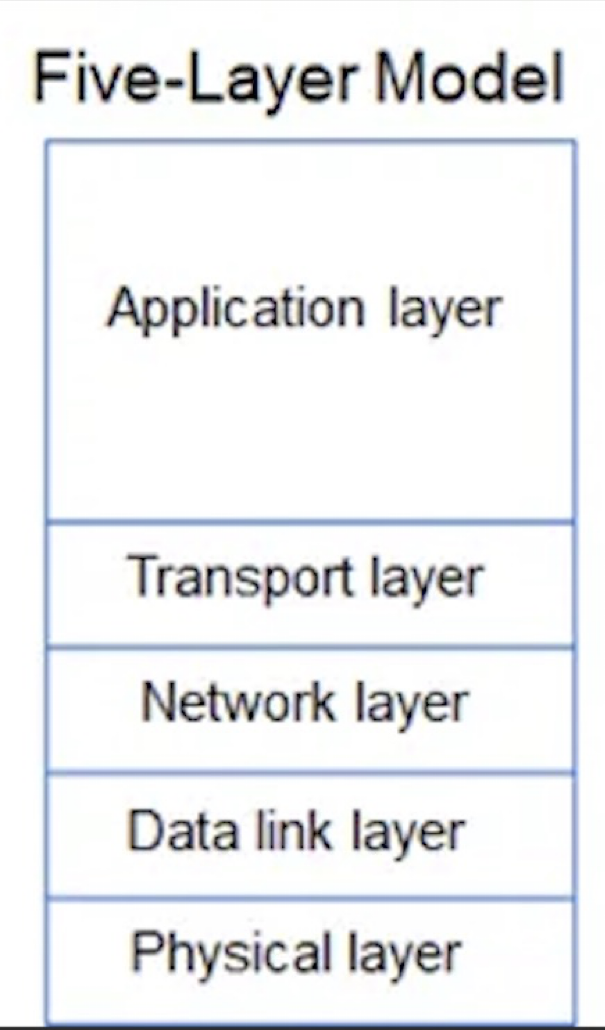
\includegraphics[scale = 0.2]{5_layer_model.png}
\caption{5-layer network model.}
\label{fig:5-layer}
\end{figure}

A computer network appears to be doing a million things all at once: gathering user input, routing data, signaling, addressing each computer, parsing data, etc. Network models are a helpful tool to break down and untangle this mess into different processes that communicate with each other. We used the 5-layer network model, seen in Figure \ref{fig:5-layer}, to help us understand how the Internet is set up. 

The foundation for any network model is the physical layer. This layer has one main responsibility: to transmit a raw bit of data. Every machine must also be able to read in its current state (high or low voltage). If the connection between machines is wired, then these bits are often represented as voltage levels, with a 0 being low voltage and a 1 being high voltage. When dealing with wireless connection, there are various modulation techniques such as analog modulation (what AM/FM radios use) or digital modulation (what WiFi uses) but they are all different approaches to the same question of how to represent one bit. In our case, we would either turn on or turn off the GPIO (General Purpose Input Output) pins on the Raspberry Pis that corresponded to the port our optic cables were connected to. We were able to use a pre-existing library for the Pi’s so we did not create the physical layer of our network. The custom made NICs did pose the biggest challenge within the physical layer as they are quite noisy and the receiving ports start in a random state. We worked around this by sending a “header” prior to sending the actual data so that we know what state the receiving pin will be in when it comes time to read in the message. The physical layer is also defined by the hardware itself, in this case the NICs, Raspberry Pis, ribbon cables, and optic cables. 

The data link layer’s main responsibility is to send frames (collection of bits) back and forth from one machine to another. This layer is where two separate, autonomous machines begin communicating with each other and sharing data. The link layer receives data from the network layer, converts it into bits that the physical layer can understand, and then divides those bits into frames, sending each frame bit-by-bit. This same process happens in reverse in the receiving machines as the link layer receives bits from the physical layer and then packages them back up into frames, parsing those frames back into the form of the original user input (for our chat feature this was text). The data link layer is also responsible for error detection, which often takes the form of redundant bits. This means that bits are added to the end of a message that somehow allow the receiving computer to know if the message has an error. There are multiple methods for this, such as checksums, parity bits, and cyclic redundancy checks, but they all involve adding on redundant bits. The receiving end is responsible for detecting errors. When an error is detected, a link layer can either attempt to fix the error before sending it up to the network layer or it can request the information to be sent again. The fastest rate at that bits can be sent is also decided in the link layer. This is often referred to as ‘bps’ which stands for bits per second. 

\begin{figure}[ht]
\centering
\includegraphics[scale = .4]{net_top.png}
\caption{Common network topologies.}
\label{fig:topologies}
\end{figure}
The network layer is the source of each computer’s spatial awareness; it says what other computers it is connected to as well as where to reach them. A network layer’s main responsibility is to transmit data from the source to the given destination without changing the data. The arrangement of machines within a network is called a Network Topology. In a network topology, the machines are referred to as nodes and different topologies are defined by how the various machines are connected. Figure \ref{fig:topologies} shows the most common kinds of topologies. Our network layer is currently implemented as a star topology; however, this could be easily switched to a ring topology with no more work than is required to run the program as is. This will be delved into deeper later in the paper when discussing the network layer. 

While a network layer does not change the user’s actual message or data that they are trying to send, it does end up sending or forwarding more than just that message. The machine that is the source of the data being sent adds on a header that is sent with (before) the message. This header consists of the source address and the destination address. When a machine receives a message, it first checks the destination address. If the destination matches the destination of the machine reading it in, then the routing is completed and the data has reached its destination. If the destinations do not match, however, then the intermediate machine must figure out how it is connected to the destination and forward the message onto that panel. In this checking process, it is crucial that the message is not altered. The network layer also works with the data link layer to control the flow of data and prevent congestion. Congestion occurs when a machine is attempting to send data either faster than the link layer’s support data flow rate or faster than the speed at which the receiving machines can process the input.

As seen in Figure \ref{fig:5-layer}, there are two more layers on top of the network layer: the transport and application layers. The transport layer is essentially abstracting and protecting everything that is happening beneath it. In some implementations, it is also responsible for ensuring that the message was successfully delivered. The application layer is then on top of this entire structure and is what us, as users of the modern internet, are most familiar with. This is where the sending of bits goes beyond bits and becomes cat videos, checking the weather, and calling your mom. In our implementation, the responsibilities of the transport layer are taken on by the network layer, creating what is essentially a 4 layer network model: physical, link, network, and application. 

\section{Link Layer}
The link layer is nestled between the physical and network layers and it is where the grunt work of data transmission and receiving happens. The fundamental question answered by the link layer is: how can one send data when their only capability is flipping a switch (in our case a GPIO pin)? This process is called encoding. There are basic styles of encoding, such as NRZ (Non-Return to Zero), where low voltage represents 0 and a high voltage represents a 1. While this style of encoding is straightforward, it also opens up the network to potentially misinterpreted data fairly easily. If the receiver's clock gets out of sync with the sender's clock, then it could miss intermediate bits, thus changing the entire message. This means that along with the bits being sent, some kind of clock signal must be sent over the machines as well. Largely because of this flaw, we chose to implement Manchester Encoding in our link layer instead. In Manchester Encoding, edges between voltage levels, rather than the levels themselves, are what represents a bit. As is common with Manchester Encoding, a rising edge (transition from low to high voltage)  represents a 0 and a falling edge (high to low voltage) represents a 1. This does mean that the bps (bits for second) for networks using Manchester encoding is half of those using something like NRZ, as the sending of one bit requires two logic states. However, by combining the clock cycle and data into one stream it is much easier to synchronize two machines. On the receiving end, we utilized the pigpio library’s callback function. This function allowed us to assign a listener to certain pins (in our case receiving pins) and we gave that listener a set of instructions to perform every time a change in state was detected on that pin. This pre-written function worked seamlessly with Manchester Encoding. The timing between edges is crucial, as it determines if the bit is ‘valid’ and should be read as data or not. A major challenge that stumped us for a while was our timing was consistently inconsistent. After lots of trials, we discovered that the timing of a rising edge versus a falling edge is slightly different. Thus, we needed a base time for each to compare every following edge to. We got these base time values by sending a header. Prior to every message, the sender’s machine would send {0, 1, 0, 1} which gave enough edges for the receiver’s callback to set a base time for a falling edge and one for a rising edge. This way, when the message itself started coming through the receiver only had to wait for a level change, see how long between this level change and the last one, and depending on that number either add it to the final received result or throw it out and wait for the next one. 
Besides the sending and receiving of data, the link layer must also perform error detection and some kind of correction. This is necessary for all link layers but is especially crucial in ours as the custom NICs are quite noisy. In our implementation, we do not have any kind of director error correction and instead, when an error is detected, we signal to the computer that sent the corrupted message that an error was detected and requests it to send the message again. This is called backwards error correction. However, our code does not implement true backwards error correction as, when an error is detected, the sending machine does not automatically re transmit the last message. Instead, a message prompts the user saying that an error was detected and requests them to type in their last message again. This means that, theoretically, the user could see this message and, for some unknown reason, send an entirely different message and the original message would be forever lost and inaccessible to the receiver. This backwards error correction process is one shared between the network and link layer. 


\section{Network Layer}
Building upon the foundation provided by the physical and link layers, the network layer is where networks become the interconnected web we are all familiar with. If there was just a link layer, then everyone you wanted to send a cat video to would be directly connected to your machine via some sort of cable. With a network layer, however, you just need the address of your destination and the web can forward your message along until it arrives at the destination. What this web looks like is determined by the network’s topology and choosing which one to implement was one of the biggest design decisions we made in our network. Currently, our network can support both ring and star topology but we have been mostly just using a star topology.
We chose to stick with the star topology as it is more robust than a ring topology. In a ring topology, if one link is severed then the whole network is done. However, in a star topology only the node connected to the failed link is affected. The stakes, however, are much higher if the “hub” (node in the middle of the star), fails as then the whole network will crash down. Troubleshooting in star topology is also easier. This was important to us as we ended up doing lots of troubleshooting in our network layer. Local area networks (LAN) are often set up in star topology. Our network layer that is currently implemented is rudimentary. It requires each machine’s ‘network\_layer.c’ file to be manually updated before running to represent the map. 
\begin{figure}[ht]
\centering
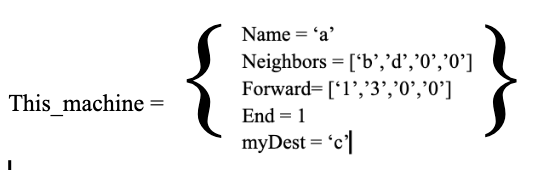
\includegraphics[scale = .4]{fig_3.png}
\caption{Node Setup}
\label{Network Toplogy}
\end{figure}

Figure 3 shows you what the fields that the user must input into look like. The ‘name’ field represents that machines address, ‘neighbors’ holds the addresses of every machine that this machine is connected to, ‘forward’ says at which port is this machine connected to its neighbors (i.e. if neighbors = {‘mach1’, ‘mach2’, 0, 0} and forward = {3, 1, 0, 0} then this machine is connected to a machine with the address mach1 on port 3 and one with the address mach2 on port 1). The last field ‘end’ can either be a 1 or a 0, indicating if it is an “end” node in the star topology or a 0 if it is the middle one. This is because in a star topology only the end nodes are interacted with by the user and the middle node is solely responsible for transporting. If one wanted to use our network layer implementation to support a ring topology, then every node would be set to be an end node as every node in a ring topology is an autonomous machine meant to take in user data/input. 
Our current addressing technique is a limitation within our network layer as it is currently set up to just be represented with one char, meaning there could only be 256 machines connected. If you set up our network with the ring topology, it can support as many pi/NIC pairs that one has access to. However, in the star topology it can only support up to 5 machines, with 4 of them communicating as the middle “hub” can be connected to max 4 machines as it only has 4 ports. 
Beyond checking and forwarding the message through the network, the network layer on the source’s machine adds a kind of header to the message. It adds on first its own source address as well as its destination address. This header is not to be confused with the header required by our link layer, as that is sent prior to each message as well but it is just for timing purposes and contains no real data. The destination address is checked by every machine upon receiving to see if it has reached its final destination or if it must be forwarded. Currently, the extent of our path finding is represented in figure 3, with the indices of the neighbors and the indices of the ports matching. This works with star topology as only the middle node needs to know where the paths are and every machine simply has to send to or receive from one node (the one connecting them to the middle). This is also incredibly simple with ring topology, as no path finding is required with every node only being connected to one other. If we were to expand our network into one that more closely reflects the Internet now, we would need to implement much more advanced path finding algorithms to ensure a) that data could be sent from one “network bunch” to another without having a full picture of every single “network bunch” and its connections and b) that the data was always taking the shortest possible path to its destination. 
The network layer must also ensure that the data is flowing through the network at a rate readable by the link layer. This was a difficult problem to solve as any time a user attempted to type a message into the chat before the previous chat was done being sent, the machines would get quite confused and bad things would happen. This was unfriendly to the user as they had no way to even know when the first message had been sent. We ended up solving this error by implementing a queue within each machine. Each machine has a messages queue and rather than actually sending data every time the user attempts to, it merely adds that data to the queue of data that has to be sent. Then, we have an entirely separate thread that is solely responsible for checking the queue and sending a message if it is in there, removing it from the queue, and checking the queue again (repeat ad infinitum). This essentially just means that the user can add to the queue of data at any speed they want without affecting what data is actually being sent across connections and at what time. We originally implemented a received data queue as well, but then realized that if the data is being sent at a controlled rate then it will be received at one as well. Besides, the raspberry pi’s have single threaded CPU cores and only 4 cores each so we needed to be selective with what process were to be threaded individually. Additionally, the more threads involved in the network layer the more possibilities for inconsistent and difficult to debug errors. 


\section{Applications}
The application layer is what most of us think of when we think of the internet. In fact, it is what most of us think of when we think of programming. All high level programming languages, such as Python and Java, abstract the machine instructions away from the programming and take that compile step for them. When the package or data reaches its final destination, checked by the network layer, it gets passed up to the application where, depending on the application, some action is performed. Looking back, we had been taking shortcuts in our model and lumping the application into the other layers by converting bits into characters and vice versa. This is a chat application. However, it is a very rudimentary one. We attempted to expand beyond this and create a multiplayer battleship game, coupled with an interactive storytelling platform and visuals. We successfully coded this in C on one computer. However, when we attempted to add this onto our existing network an dlink layers, it was not successful. We think that this is because we structured much of our code around chat features that pivoting to game moves affected the behavior. We did not have enough time to pin down the source of the errors and thus, our only application at the end of the class was the chat feature. 

\section{Future Work}
With only 3.5 weeks to build up an entire network model from nearly scratch, there are nearly endless options for what we would do if we had more time. Starting with our network layer, we would potentially revert back to using the waveform functions within the pigpio library as that could maybe fix some timing errors we were having as all the waves are first created and then sent at once, as opposed to created and sent one by one. Moving up to the network layer, we would store the last sent message so that when an error is detected, the machines can communicate without the user having to manually re-input their last message. We would also expand our mapping strategies to be more dynamic and expandable. This means that when connections are broken or created mid-way through running the program, the individual machines adapt and update their routing tables. Then, with a robust and reliable network layer with a strong foundational link layer, we would return to and conquer battleship. 
\section{Conclusion}
Attempting to create and build an alternative to the standard Internet was a tumultuous process, to say the least. As mentioned, we began with limited exposure to any hardware and an understanding of the C programming language,  but not quite a proficiency. 
If we were to do the problem again we would change our angle of approach. In the future focusing more on robust testing before moving onto the next stage of the problem would have fixed many of the issues that we encountered. Having the final application layer in mind when constructing the link and network layers would have decreased our tech debt and made the movement between layers much more fluid. 
Beyond the actual content itself, this was both of our first timing solving an essentially unsolved computational problem. But bit by bit, a bit becomes a byte. This process was a balance of doing thorough research yet also accepting an endless cycle of trial and error. We grew in our team dynamic as well, learning to trust and rely on each other. While there were moments where we would break off and individually research the different aspects that our network would need, all of our code and processes are equally understood by both of us. 
\cite{cats-lasers,CP341-final,E-design,free-code-camp,gforg-ascii,gforg-manch,NRZ-Community,NRZ-unit-2,NRZ-Vikra}
\bibliographystyle{acm}
\bibliography{refs.bib}

\end{document}


